\documentclass{article} % For LaTeX2e
\usepackage{nips15submit_e,times}
\usepackage[hidelinks]{hyperref}
\usepackage{graphicx}
\usepackage[utf8]{inputenc}
\usepackage{float}
\usepackage{url}
%\documentstyle[nips14submit_09,times,art10]{article} % For LaTeX 2.09


\title{CCA-based Multi-View Learning to Improve Cross-lingual Retrieval}






% The \author macro works with any number of authors. There are two commands
% used to separate the names and addresses of multiple authors: \And and \AND.
%
% Using \And between authors leaves it to \LaTeX{} to determine where to break
% the lines. Using \AND forces a linebreak at that point. So, if \LaTeX{}
% puts 3 of 4 authors names on the first line, and the last on the second
% line, try using \AND instead of \And before the third author name.

\newcommand{\fix}{\marginpar{FIX}}
\newcommand{\new}{\marginpar{NEW}}

%\nipsfinalcopy % Uncomment for camera-ready version

\begin{document}
	
	
	\maketitle
	
	\begin{abstract}
		In Cross-Language Information Retrieval, finding the appropriate translation of the source language query has always been a difficult problem to solve. We use the CCA to project the  vector space model of the words from two different languages onto the same space. We make us of the Canadian Hansard datasets consisting of two languages - English and French.
	\end{abstract}
	
	\section{Introduction}
	
	Since it's the age of globalization, dealing with multi-lingual documents is a very relevant problem in everyday's life. Naturally, developing and improving the computational and analytical tools for multi-language documents processing is an active area of research. Many work in the literature have been reported addressing the same problem. In this work, we are going to study and analyze one such method based on Canonical correlation analysis (CCA).
	
	One very simple approach to this multi-lingual document processing problem could be to append the word representation of translation of the word in other language with the representation of the original word in one language. Some of the obvious drawbacks in this approach is that the word representation becomes of higher dimension and some of the words in a language may not have exact translation in the other language.
	
	Another approach which overcomes these difficulties is the following. Intuitively, the word representations in two different language space can be projected on to a common latent space and measuring the distance between these two projected data in common space, the similarity or dissimilarity between the words can be decided. This is the simplified idea behind CCA-based approach, which has been studied and experimented in this work.
	
	This work has three separate sections. In this first section, the appropriate word embeddings have been created from the documents in different languages. Once the word representation vectors have been created, in the later section, the representations are projected on a common space using CCA, such that in the projected space, the similar words have maximum correlation. In the final section, the distance between the projected word representations have been computed in the latent space and accordingly the similar words have been retrieved.
	
	The rest of the report has been organized as follows.
	
	
	%%NIPS requires electronic submissions.  The electronic submission site is  
	%%\begin{center}
	%   \url{http://papers.nips.cc}
	%\end{center}
	
	%Please read carefully the
	%instructions below, and follow them faithfully.
	%\subsection{Style}
	
	%Papers to be submitted to NIPS 2015 must be prepared according to the
	%instructions presented here. Papers may be only up to eight pages long,
	%including figures. Since 2009 an additional ninth page \textit{containing only
	%cited references} is allowed. Papers that exceed nine pages will not be
	%reviewed, or in any other way considered for presentation at the conference.
	%This is a strict upper bound. 
	
	%Please note that this year we have introduced automatic line number generation
	%into the style file (for \LaTeXe and Word versions). This is to help reviewers
	%refer to specific lines of the paper when they make their comments. Please do
	%NOT refer to these line numbers in your paper as they will be removed from the
	%style file for the final version of accepted papers.
	
	%The margins in 2015 are the same as since 2007, which allow for $\approx 15\%$
	%more words in the paper compared to earlier years. We are also again using 
	%double-blind reviewing. Both of these require the use of new style files.
	
	%Authors are required to use the NIPS \LaTeX{} style files obtainable at the
	%NIPS website as indicated below. Please make sure you use the current files and
	%not previous versions. Tweaking the style files may be grounds for rejection.
	
	%% \subsection{Double-blind reviewing}
	
	%% This year we are doing double-blind reviewing: the reviewers will not know 
	%% who the authors of the paper are. For submission, the NIPS style file will 
	%% automatically anonymize the author list at the beginning of the paper.
	
	%% Please write your paper in such a way to preserve anonymity. Refer to
	%% previous work by the author(s) in the third person, rather than first
	%% person. Do not provide Web links to supporting material at an identifiable
	%% web site.
	
	%%\subsection{Electronic submission}
	%%
	%% \textbf{THE SUBMISSION DEADLINE IS June 5, 2015. SUBMISSIONS MUST BE LOGGED BY
	%% 23:00, June 5, 2015, UNIVERSAL TIME}
	
	%% You must enter your submission in the electronic submission form available at
	%% the NIPS website listed above. You will be asked to enter paper title, name of
	%% all authors, keyword(s), and data about the contact
	%% author (name, full address, telephone, fax, and email). You will need to
	%% upload an electronic (postscript or pdf) version of your paper.
	
	%% You can upload more than one version of your paper, until the
	%% submission deadline. We strongly recommended uploading your paper in
	%% advance of the deadline, so you can avoid last-minute server congestion.
	%%
	%% Note that your submission is only valid if you get an e-mail
	%% confirmation from the server. If you do not get such an e-mail, please
	%% try uploading again. 
	
	
	%\subsection{Retrieval of style files}
	
	%The style files for NIPS and other conference information are available on the World Wide Web at
	%\begin{center}
	%  \url{http://www.nips.cc/}
	%\end{center}
	%The file \verb+nips2015.pdf+ contains these 
	%instructions and illustrates the
	%various formatting requirements your NIPS paper must satisfy. \LaTeX{}
	%users can choose between two style files:
	%\verb+nips15submit_09.sty+ (to be used with \LaTeX{} version 2.09) and
	%\verb+nips15submit_e.sty+ (to be used with \LaTeX{}2e). The file
	%\verb+nips2015.tex+ may be used as a ``shell'' for writing your paper. All you
	%have to do is replace the author, title, abstract, and text of the paper with
	%your own. The file
	%\verb+nips2015.rtf+ is provided as a shell for MS Word users.
	
	%The formatting instructions contained in these style files are summarized in
	%sections \ref{gen_inst}, \ref{headings}, and \ref{others} below.
	
	%% \subsection{Keywords for paper submission}
	%% Your NIPS paper can be submitted with any of the following keywords (more than one keyword is possible for each paper):
	
	%% \begin{verbatim}
	%% Bioinformatics
	%% Biological Vision
	%% Brain Imaging and Brain Computer Interfacing
	%% Clustering
	%% Cognitive Science
	%% Control and Reinforcement Learning
	%% Dimensionality Reduction and Manifolds
	%% Feature Selection
	%% Gaussian Processes
	%% Graphical Models
	%% Hardware Technologies
	%% Kernels
	%% Learning Theory
	%% Machine Vision
	%% Margins and Boosting
	%% Neural Networks
	%% Neuroscience
	%% Other Algorithms and Architectures
	%% Other Applications
	%% Semi-supervised Learning
	%% Speech and Signal Processing
	%% Text and Language Applications
	
	%% \end{verbatim}
	
	\section{Related Work}
	\label{related_work}
	In this section, some of the related work mentioned in the literature have been explained in brief. In \cite{Gong2013}, the 3-view Kernel CCA has been used for modeling Internet images. In this work, the data has been taken into a common latent space using CCA and a similarity function has been computed between pairwise projected data in latent space for modeling and tagging. The authors have experimented using Flickr-CIFAR, NUS-WIDE and INRIA-websearch datasets.
	
	In \cite{Faruqui2014}, the authors have mentioned an improvement of word vector representation using CCA-based approach for multi-lingual data. The intuition behind this work is that the lexico-semantic content are invariant across languages. The authors have presented their results on several datasets including WMT-2011 (English, German, Spanish), combined WMT-2011 and 2012 (French). The results of the proposed word representation in this work has also been compared with several other existing word representations, as Singular value decomposition (SVD) vectors, recurrent neural network (RNN) vector, Skip-gram (SG) vector etc.
	
	A multi-lingual clustering approach has been used in \cite{Bhattacharya2016} for cross-language query translations and it has been reported that the method performs better than the dictionary-based methods. The results have been obtained using FIRE 2012 and Wikipedia datasets. The authors have reported that this method works best when combined with dictionary and Google translates in hybrid model.
	
	
	\section{Dataset description}
	\label{dataset}
	For this work the dataset has been used is Hansard record of Parliamentary documents \cite{datalink}. It contains aligned text data from official records of $36^{th}$ Canadian Parliament. 
	
	
	\section{Baseline Experiments}
	\label{experiment}
	
	In this section, the experiment to demonstrate the CCA-based multi-lingual text retrieval has been explained.
	\subsection{Word Embedding}
	Vector space model is well known in information retrieval where each document is represented as a vector. The vector components represent weights or importance of each word in the document.
	
	Although the idea of using vector representation for words also has been around for some time, the interest in word embedding, techniques that map words to vectors, has been soaring recently. One driver for this has been Tomáš Mikolov’s Word2vec algorithm which uses a large amount of text to create high-dimensional (50 to 300 dimensional) representations of words capturing relationships between words unaided by external annotations. Such representation seems to capture many linguistic regularities. For example, it yields a vector approximating the representation for vec(‘Rome’) as a result of the vector operation vec(‘Paris’) – vec(‘France’) + vec(‘Italy’).
	
	The word2vec algorithm uses a fully connected Neural Network to generate vectors for words as shown below. The input layer contains as many nodes as there are unique words in the document. The output layer also has the same number of nodes as the input layer. The hidden layer has a linear activation function. The number of nodes in the hidden layer should be equal to dimension of the vector we want for each word.Thus, assuming that the vocabulary for learning word vectors consists of $V$ words and $N$ to be the dimension of word vectors, the input to hidden layer connections can be represented by matrix $WI$ of size $VxN$ with each row representing a vocabulary word. In same way, the connections from hidden layer to output layer can be described by matrix $WO$ of size $NxV$. In this case, each column of $WO$ matrix represents a word from the given vocabulary. The input to the network is encoded using “1-out of -V” representation meaning that only one input line is set to one and rest of the input lines are set to zero.
	
	$WI$ will be our word2vec matrix after the training is complete.
	
	\begin{figure}[H]
		\begin{center}
			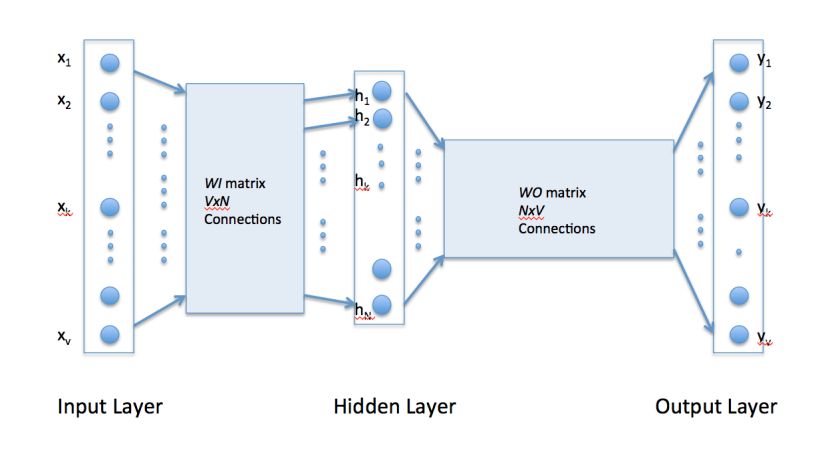
\includegraphics[scale = 0.6]{Figures/word2vecNN.png}
			\caption{Word2vec Neural Network Trainer}
			\label{fig:word2vecNN}
		\end{center}
	\end{figure}
	
	\subsection{Canonical Correlation Analysis (CCA)}
	
	Canonical correlation analysis (CCA) is a method for exploring the relationships between two multivariate sets of variables (vectors) by making sense of cross-covariance matrices.
	\\\\
	{\bf Definition}\\
	Given two column vectors $\bf{{X} = (x_1, x_2,..., x_n)'}$ and  $\bf{{Y} = (y_1, y_2,..., y_n)'}$ of random variables with finite moments, one may define the cross-covariance ${\Sigma_{XY}} = cov({X},{Y})$ to be a ${{\bf n}\times{\bf m}}$ matrix whose (i,j) entry is the covariance $cov(x_i,y_j)$.\\
	In practice the covariance matrix is estimated based on the sampled data $\bf{X}$ and $\bf{Y}$.\cite{ccadefn}
	
	
	Canonical correlation seeks vectors ${a}$ and ${b}$ such that the random variables $\bf{a'X}$ and $\bf{b'Y}$ maximize the correlation coefficient ${\bf \rho}$.
	
	\begin{equation}
	(a,b) = \arg \max_{(a,b)} {\rho}({a'X},{b'Y}).
	\end{equation}
	where,
	\begin{equation}	
	\rho({a'X},{b'Y}) = \frac{a' \Sigma_{XY} b}{\sqrt{a'\Sigma_{XX}a}\sqrt{b'\Sigma_{YY}b}}	
	\end{equation}
	
	The random Variables $\bf{U_1 = a'X}$ and $\bf{V_1 = b'Y}$ are the first pair of canonical variables.
	
	In general, the $\bf{k^{th}}$ pair of canonical variables are the linear combinations $(\bf{U_k,V_k})$ that maximize the correlation coeeficient $\bf{\rho}(\bf{U_k,V_k})$ among all possible linear combinations and are uncorrelated with the previous $\bf{(k-1)}$ canonical variables.\\
	This procedure may be continued upto {\bf{min (m,n)}} times.\cite{ccaimpl}
	
	Canonical correlation analysis finds practical importance in the areas of supervised learning, clustering, dimensionality reduction, reinforcement learning etc.
	
	\begin{figure}[H]
		\begin{center}
			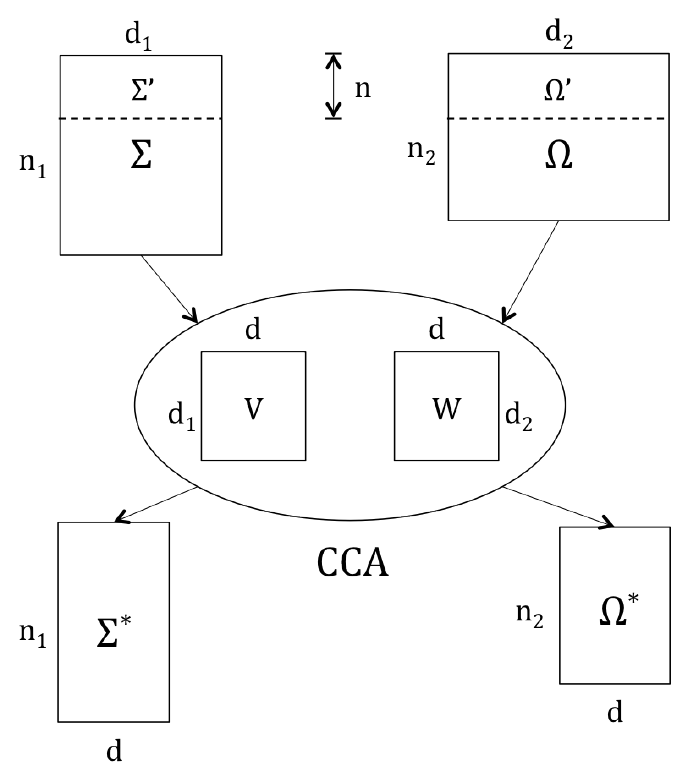
\includegraphics[scale = 0.6]{Figures/cca.png}
			\caption{Cross-lingual word vector projection using CCA	}
			\label{fig:CCA_implementation}
		\end{center}
	\end{figure}
	
	In our implementation of CCA we are considering two subspaces of the original space and reducing the dimensionality by projecting onto a common dimension using CCA.(Figure \ref{fig:CCA_implementation})
	
	
	\section{Future Work}
	The future direction of work for this project has been identified as follows.
	\begin{itemize}
		\item Since CCA can be kernelized and the possibility of performance of kernelized version CCA is better, the word retrieval results obtained using CCA can be compared with the Kernelized-CCA based cross-lingual word retrieval to observe the improvement of performance.
		\item Different word embedding techniques can be used for extracting text features and their performances for each case can be compared.
		\item The length of the projected CCA-vector dimensions may be varied and compared to find out the optimal projected feature length in the latent space required for this particular application.
		\item The next course of action would be to look into the possibility of unifying the above mentioned algorithms into one super-algorithm that enhances the performance of the multi-lingual translation problem. This can be achieved by appropriate prioritization of the different algorithms.
	\end{itemize}
	
	
	
	%\subsection{Figures}
	
	%\begin{figure}[h]
	%\begin{center}
	%\framebox[4.0in]{$\;$}
	%\fbox{\rule[-.5cm]{0cm}{4cm} \rule[-.5cm]{4cm}{0cm}}
	%\end{center}
	%\caption{Sample figure caption.}
	%\end{figure}
	
	\section{Conclusion}
	To conclude, in this project, so far, the literature review has been performed and the understanding of the algorithms at theoretical and implementation level has been performed. 
	
	
	%\begin{table}[t]
	%	\label{sample-table}
	%	\begin{center}
	%		\begin{tabular}{ll}
	%			\multicolumn{1}{c}{\bf PART}  &\multicolumn{1}{c}{\bf DESCRIPTION}
	%			\\ \hline \\
	%			Dendrite         &Input terminal \\
	%			Axon             &Output terminal \\
	%			Soma             &Cell body (contains cell nucleus) \\
	%		\end{tabular}
	%	\end{center}
	%\end{table}
	
	
	
	%\subsubsection*{Acknowledgments}
	
	%Use unnumbered third level headings for the acknowledgments. All
	%acknowledgments go at the end of the paper. Do not include 
	%acknowledgments in the anonymized submission, only in the 
	%final paper. 
	
	%\subsubsection*{References}
	
	
	\begin{thebibliography}{1}
		
		\bibitem{Gong2013}
		Y. Gong, Q. Ke, M. Isard \& S. Lazebnik, (2013) A multi-view embedding space for modelling internet images, tags and their semantics. In {\it International Journal of Computer Vision}, {\bf 106}(2):210-233.
		
		\bibitem{Faruqui2014}
		M. Faruqui \& C. Dyer (2014) Improving vector-space word representation using multi-lingual correlation. In {\it Proc. European Chapter of the Association for Computational Linguistics}.
		
		\bibitem{Bhattacharya2016}
		P. Bhattacharya, P. Goyal \& S. Sarkar (2016) Query translation for cross-language information retrieval using multi-lingual word cluster. In {\it Proc. South and Southeast Asian Natural Languages Processing}.
		
		\bibitem{datalink}
		Dataset Link : \url{http://www.isi.edu/natural-language/download/hansard/}

		\bibitem{ccadefn}
		Link : \url{https://onlinecourses.science.psu.edu/stat505/node/63}

		\bibitem{ccaimpl}
		 Link : \url{https://en.wikipedia.org/wiki/Canonical_correlation}
		
	\end{thebibliography}
	
	
\end{document}
